%% amssamp1.tex is nearly lidentical to amssamp2.tex, except
%% that amssamp2.tex uses the [twocol] option to produce
%% two-column text. Note that the figures and tables need to be
%% placed in text nearthe first callout, not at the end of the 
%% document. Also note that star form is used for figures
%% and tables.
\documentclass[twocol]{ametsoc}

%%%%%%%%%%%%%%%%%%%%%%%%%%%%%%%%
%%% To be entered only if twocol option is used
\journal{jtech}

%  Please choose a journal abbreviation to use above from the following list:
% 
%   jamc     (Journal of Applied Meteorology and Climatology)
%   jtech     (Journal of Atmospheric and Oceanic Technology)
%   jhm      (Journal of Hydrometeorology)
%   jpo     (Journal of Physical Oceanography)
%   jas      (Journal of Atmospheric Sciences)	
%   jcli      (Journal of Climate)
%   mwr      (Monthly Weather Review)
%   wcas      (Weather, Climate, and Society)
%   waf       (Weather and Forecasting)
%   bams (Bulletin of the American Meteorological Society)
%   ei    (Earth Interactions)

%%%%%%%%%%%%%%%%%%%%%%%%%%%%%%%%
%Citations should be of the form ``author year''  not ``author, year''
\bibpunct{(}{)}{;}{a}{}{,}

\title{Smoothing Noisy GPS Data with Tension}

\authors{Jeffrey J. Early\correspondingauthor{Jeffrey J. Early, NorthWest Research Associates, 
				4118 148th Ave NE, Redmond, WA 98052.} and Adam Sykulski}

\affiliation{NorthWest Research Associates} 

\email{jearly@nwra.com}

\abstract{We develop a technique for smoothing noisy GPS data using B-splines with tension. We show how the tension condition routinely employed in smoothing splines can be restated as a maximum likelihood problem and then how the tension parameter can be chosen based on physical reasoning. The GPS errors appear to be non-Gaussian, so we use a t-distribution in the maximum likelihood.  }


\begin{document}

\maketitle

%%%%%%%%%%%%%%%%%%%%%%%%%%%%%%%%%%%%%%%%%%%%%%%%%%%%%%%%%%%%%%%%%%%%%
% MAIN BODY OF PAPER
%%%%%%%%%%%%%%%%%%%%%%%%%%%%%%%%%%%%%%%%%%%%%%%%%%%%%%%%%%%%%%%%%%%%%
\section{Introduction}
Global positioning system receivers (now commonly referred to as `a GPS') are used in literally billions of devices around the the world to track positions. The quality of the position data can be quite good, with accuracies down to a few meters (cite gps.gov), but real world effects (such as atmospheric conditions sky blockages, to quote gps.gov) can significantly increase the errors. Kalman filters are often employed to reduce these errors because they can be run in real time (cite something). Here we consider an alternative approach using smoothing B-splines to control errors for data that has been collected and archived.

The data shown here was collected from from oceanic surface \emph{drifters}, floating buoys with drogues tethered 15-30 meters below the ocean surface, depending on the particular experiment. In the past, these drifters have used Argos positioning system which has significantly poorer temporal coverage and position accuracy (cite elipot), but recently more surface drifters have employed GPS receivers and transmitted their data back through Argos or Iridium satellites. The GPS receiver sits on the surface buoy and collects position data, but because of atmospheric conditions or ocean waves, the receivers are sometimes unable to obtain a position, or when they do, it is highly inaccurately. Thus, despite nominal accuracies of a few meters, it is often the case that some positions are off by more than 1000 meters.

In addition to correcting the position errors, it is also important to interpolate the data to a regular grid. Although the sampling period of a GPS receiver can be fixed, because of missing data and time to to acquire signals, the sampling can be quite irregular. Because many analysis techniques require regular sampling (e.g., a Fourier transform), it is necessary to interpolate the signal onto a regular grid. So the approach taken here is not to simply discard poor data, but also to interpolate the position.

For this particular note we will consider nine surface drifters that were deployed in the Sargasso Sea in the summer of 2011. These particular drifters were part of the LatMix experiment (cite BAMs) and recorded data at approximately 30 minute intervals over the course of a week before being retrieved.

The drifter positions are bivariate time series data given as either projected coordinates $(x_i, y_i)$ or longitude/latitude $(\phi_i, \theta_i$) at times $t_i$. The goal is to create a model of position $(x(t),y(t))$ that is continuous in $t$, and perhaps even continuous a higher derivative---such as velocity or acceleration---that best matches the data given an assumed set of errors. Conceptually this task can be divided into two parts, \emph{interpolating} the data to a continuous time series and \emph{smoothing} the data to remove the noise in the positions.

%%%%%%%%%%%%%%%%%%%%%%
%
\section{Interpolation}
%
%%%%%%%%%%%%%%%%%%%%%%

\begin{figure*}[t]
  \centerline{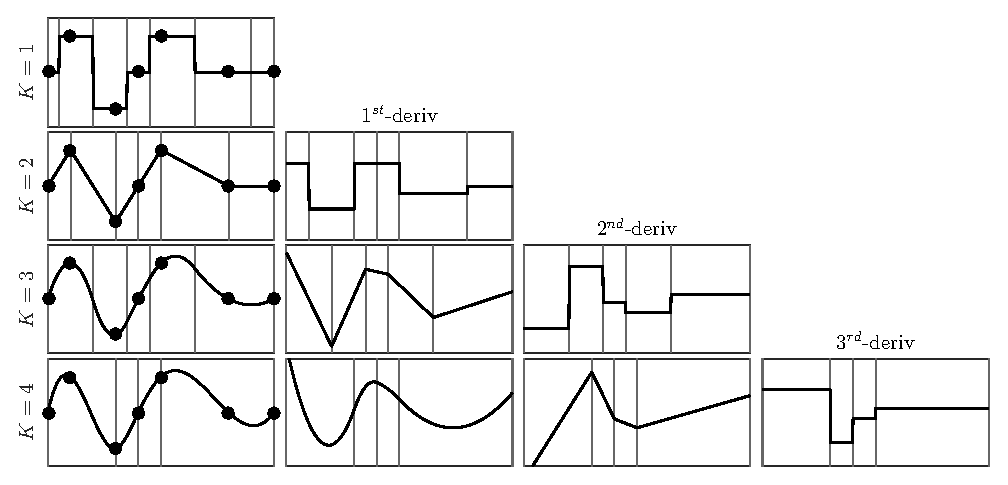
\includegraphics[width=39pc,angle=0]{interpolation}}
  
  \caption{This shows an example of interpolating between 7 data points. The data points are shown as circles, and the interpolated function is shown as a solid black lines. We show four different orders of interpolation $K=1..4$ (rows) and their nonzero derivatives (columns). The thin vertical grey lines are the knot points.}
  \label{interpolation}
\end{figure*}

Assume for the moment that we are given $N$ observations of a particle position $(t_i,x_i)$ with no errors. The simplest possible form of interpolation would be a nearest neighbor method that assigns the position of the particle to the nearest observations in time. The resulting interpolated function $x(t)$ is a polynomial of \emph{order} $K=1$ (piecewise constant), shown in the top row of figure \ref{interpolation}. The next level of sophistication is to assume a constant velocity between any two observations and use that to interpolate positions between observations, second row of figure \ref{interpolation}. This also means that we now have a piecewise constant function $\frac{dx}{dt}$ that represents the velocity of the particle, shown in the second row, second column of figure  \ref{interpolation}. This is a polynomial function of order $K=2$.

It is slightly less obvious how to proceed to a polynomial of order $K=3$. Clearly we want a piecewise constant acceleration (the second derivative), but where to place $\emph{knot points}$ that define the boundaries of the regions  and how to maintain continuity is slightly less clear. The approach taken here is to use B-splines.

%%%%%%%%%%%%%%%%%%%%%%
\subsection{B-Splines}
%%%%%%%%%%%%%%%%%%%%%%

A B-spline (or basis spline) of \emph{order} $K$ (\emph{degree} $S=K-1$) is a piecewise polynomial that maintains nonzero continuity across $S$ knot points. The knot points are a nondecreasing collection of points in time that we will denote with $\tau_i$. The basic theory is well documented in (cite de Boor), but here we will present a reduced version specifically tailored to our needs.

The $m$-th B-spline of order $K=1$ is defined as,
\begin{equation}
X^1_m(t) \equiv \begin{cases}
1      & \text{if $ \tau_m \leq t < \tau_{m+1}$}, \\
0     & \text{otherwise}.
\end{cases}
\end{equation}
This is the rectangle function as shown in the first row, first column of figure \ref{bsplines}. If we are given $P$ knot points, then we can construction $P-1$ B-splines of order $K=1$, although notice that if a knot point is repeated this will result in a splines that is zero everywhere. To represent an interpolating function $x(t)$ for the $N$ observations of a particle position $(t_i,x_i)$ we define $N+1$ knot points as,
\begin{equation}
\tau_m = \begin{cases}
t_1      & \text{$m=1$}, \\
t_{m-1} + \frac{t_{m-1}-t_m}{2}	  & \text{$1<m \leq N$}\\
t_N     & \text{$m>N$}.
\end{cases}
\end{equation}
This will create $N$ independent basis functions that provide support for the region $t_i \leq t \leq t_N$ (provided the last spline is defined to include the last knot point). The interpolating function $x(t)$ is defined as $x(t) \equiv  X^1_m(t) \xi^m$ where the coefficients $\xi^m$ are found by solving $X^1_m(t^i) \xi^m = x^i$. The result of this process is shown in figure \ref{interpolation} for 7 irregularly spaced data points.

All higher order B-splines are defined by recursion,
\begin{equation}
X^K_m(t) \equiv \frac{t - t_m}{t_{m+K-1} - t_m} X^{K-1}_m(t) + \frac{t_{m+K}-t}{t_{m+K} - t_{m+1}} X^{K-1}_{m+1}(t).
\end{equation}
This recursion formula takes two neighboring lower order splines and ramps the left one up over its nonzero domain and ramps the right one down over its nonzero domain. The result of this process is to create splines that span across one additional knot point at each order, and maintain continuity across one more derivatives. Examples are shown in figure \ref{bsplines}.

Any knot points that are repeated $T$ times will result in an a total of $T-1$ splines of order one that are everywhere zero. This has the effect of introducing discontinuities in the derivatives for higher order splines. For our purposes, we will only use this feature to prevent higher order splines from cross the boundaries. For $K=2$ order splines we will use $N+2$ knot points at locations,
\begin{equation}
\tau_m = \begin{cases}
t_1      	& \text{$m < 3$}, \\
t_{m-1}	& \text{$3 \leq m < N$}\\
t_N 		& \text{$m \geq N$}.
\end{cases}
\end{equation}
This creates a knot point at every observation point, but repeats the first and last knot point. This has the effect of terminating the first and last spline at the boundary and creating $N$ second order B-splines, $X^2_m(t)$. Once again the interpolating function $x(t)$ is defined as $x(t) \equiv  X^2_m(t) \xi^m$ where the coefficients $\xi^m$ are found by solving $X^2_m(t^i) \xi^m = x^i$. The second row of figure \ref{interpolation} shows an example.

This process can be continued to higher and higher order B-splines. For splines that are of \emph{even} order, we create $N+K$ knots points with
\begin{equation}
\tau_m^{\text{$K$-even}} = \begin{cases}
t_1      	& \text{$m < K+1$}, \\
t_{m-K/2}	& \text{$K+1 \leq m < N$}\\
t_N 		& \text{$m>N$}
\end{cases}
\end{equation}
and for splines that are \emph{odd} order, we create $N+K$ knot points with,
\begin{equation}
\tau_m^{\text{$K$-odd}} = \begin{cases}
t_1      	& \text{$m < K+1$}, \\
t_{m-K/2} + \frac{t_{m-K/2}-t_{m-K/2+1}}{2}	& \text{$K+1 \leq m < N$}\\
t_N 		& \text{$m>N$}
\end{cases}
\end{equation}



%%%%%%%%%%%%%%%%%%%%%%
%
\section{Maximum Likelihood}
%
%%%%%%%%%%%%%%%%%%%%%%

Throughout this discussion assume that 
Slightly rewording a quote from Numerical Recipes, the central idea of maximum likelihood is to ask ``Given a particular path $(x(t),y(t))$, what is the probability that this dataset $(t_i,x_i, y_i)$ could have occurred?'' The goal is then to find the path that is most likely to have produced that dataset.

Conceptually we have two major pieces that we need to solve this problem:
\begin{enumerate}
\item we need to specify the probability function and
\item we need to specify the form of the path (model).
\end{enumerate}

%%%%%%%%%%%%%%%%%%%%%%
\subsection{Gaussian errors}
%%%%%%%%%%%%%%%%%%%%%%

The probability function is used to describe the errors in the position, $\epsilon_i \equiv x_i - x(t_i)$. The canonical example in one-dimension is to assume that the error in our position measurements are Gaussian and therefore the probability of the observed data given the model is,
\begin{equation}
\label{max-gaussian}
P \sim \prod \exp \left[ -\frac{1}{2} \left( \frac{x_i - x(t_i)}{\sigma_i} \right)^2 \right] \Delta x
\end{equation}
where $x_i$ represents the observations at time $t_i$ with estimated error of $\sigma_i$.

Maximizing the probability function in equation \ref{max-gaussian} is also the same as minimizing its argument (called the penalty function),
\begin{equation}
\label{least-squares}
\phi = \sum \left[\frac{1}{2} \left( \frac{x_i - x(t_i)}{\sigma_i} \right)^2 \right].
\end{equation}
Stated in this way is plain to see that this is the same as asking for the `least-squares' fit of the errors.

%%%%%%%%%%%%%%%%%%%%%%
\subsection{A model}
%%%%%%%%%%%%%%%%%%%%%%

Simply connecting a straight line to each individual data point would certainly maximize equation \ref{max-gaussian} (and minimize equation least-squares) because it would set all the errors to zero, but the resulting distribution of errors (a delta function at zero) wouldn't look anything like the assumed Gaussian distribution. Thus, if we want the error distribution that we get out to look like that which we assumed, it also necessary to \emph{constrain} the problem in some way. There are conceptually (at least) two ways of doing this, either 
\begin{enumerate}
\item specify a model with fewer degrees of freedom than data points, or
\item specify an additional \emph{global} constraints on the model in the penalty function.
\end{enumerate}
These two may be equivalent. For example, you may decide the model is a straight line (with two degrees of freedom), or you could set a constraint that that the integral of the second derivative vanish.

The approach taken h
\begin{figure}
  \centerline{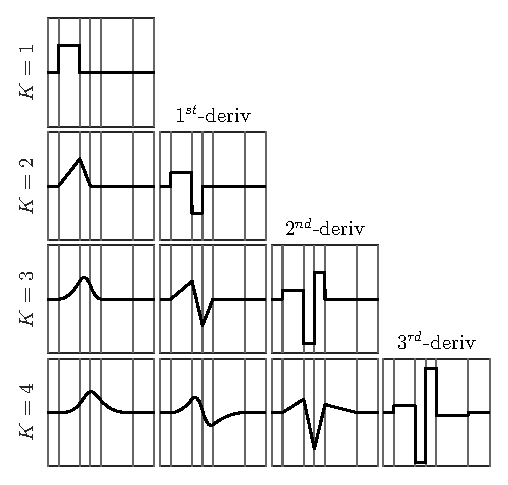
\includegraphics[width=19pc,angle=0]{bsplines}}
  \caption{This shows an example B-spline and its derivatives (columns) for orders $K=1..4$ (rows).}
  \label{bsplines}
\end{figure}




%%%%%%%%%%%%%%%%%%%%%%
%
\section{Smoothing Spline}
%
%%%%%%%%%%%%%%%%%%%%%%


%\begin{acknowledgment} 
%Start acknowledgments here.
%\end{acknowledgment}
%
%% Use appendix}[A], {appendix}[B], etc. etc. in place of appendix if you have multiple appendixes.
%\ifthenelse{\boolean{dc}}
%{}
%{\clearpage}
%\begin{appendix}
%\section*{\begin{center}Appendix Title Is Entered Here (Primary heading)\end{center}}
%\subsection{First appendix secondary heading}
%
%\subsection{Second appendix secondary heading}
%
%\subsubsection{First appendix tertiary heading}
%
%\subsubsection{Second appendix tertiary heading}
%
%\paragraph{First appendix quaternary heading}
%
%\paragraph{Second appendix quaternary heading}
%
%\end{appendix}
%
%% Create a bibliography directory and place your .bib file there.
%% -REMOVE ALL DIRECTORY PATHS TO REFERENCE FILES BEFORE SUBMITTING TO THE AMS FOR PEER REVIEW
%\ifthenelse{\boolean{dc}}
%{}
%{\clearpage}
%\bibliographystyle{ametsoc}
%\bibliography{references}
%
%%%%%%%%%%%%%%%%%%%%%%%%%%%%%%%%%%%%%%%%%%%%%%%%%%%%%%%%%%%%%%%%%%%%%%
%% FIGURES-REMOVE ALL DIRECTORY PATHS TO FIGURE FILES BEFORE SUBMITTING TO THE AMS FOR PEER REVIEW
%%%%%%%%%%%%%%%%%%%%%%%%%%%%%%%%%%%%%%%%%%%%%%%%%%%%%%%%%%%%%%%%%%%%%%
%\begin{figure}[t]
%  \noindent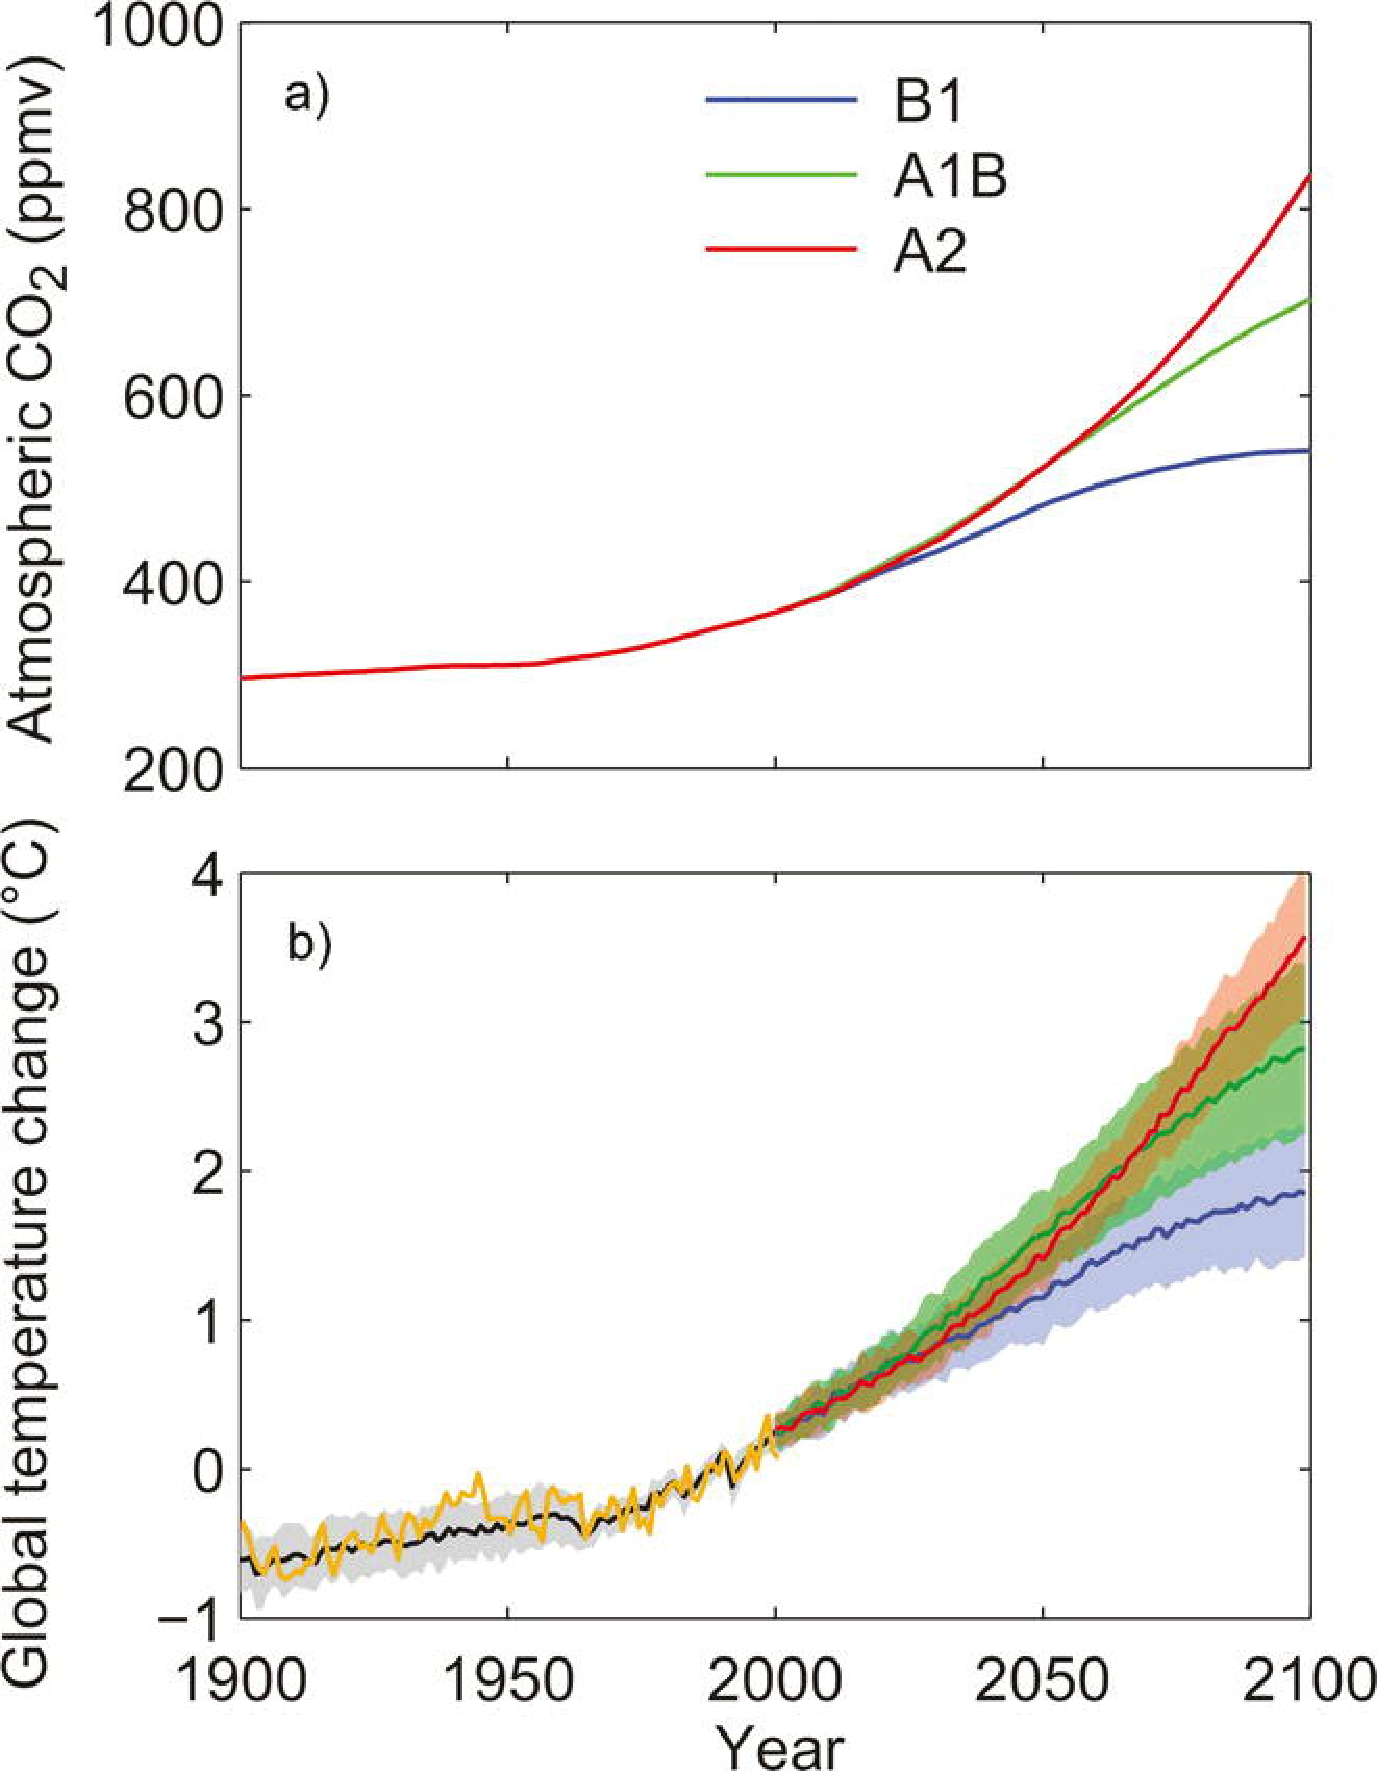
\includegraphics[width=19pc,angle=0]{figure01.pdf}\\
%  \caption{Enter the caption for your figure here.  Repeat as
%  necessary for each of your figures. Figure from \protect\cite{Knutti2008}.}\label{f1}
%\end{figure}
%%%%%%%%%%%%%%%%%%%%%%%%%%%%%%%%%%%%%%%%%%%%%%%%%%%%%%%%%%%%%%%%%%%%%%
%% TABLES
%%%%%%%%%%%%%%%%%%%%%%%%%%%%%%%%%%%%%%%%%%%%%%%%%%%%%%%%%%%%%%%%%%%%%%
%\begin{table}[t]
%\caption{This is a sample table caption and table layout.  Enter as many tables as
%  necessary at the end of your manuscript. Table from Lorenz (1963).}\label{t1}
%\begin{center}
%\begin{tabular}{ccccrrcrc}
%\hline\hline
%$N$ & $X$ & $Y$ & $Z$\\
%\hline
% 0000 & 0000 & 0010 & 0000 \\
% 0005 & 0004 & 0012 & 0000 \\
% 0010 & 0009 & 0020 & 0000 \\
% 0015 & 0016 & 0036 & 0002 \\
% 0020 & 0030 & 0066 & 0007 \\
% 0025 & 0054 & 0115 & 0024 \\
%\hline
%\end{tabular}
%\end{center}
%\end{table}
%
\end{document}